\documentclass[8pt,a4paper,landscape]{extarticle}
\makeatletter
\def\input@path{{../_shared/}}
\makeatother
\usepackage{cheatsheet}

\begin{document}

\begin{multicols*}{4}

\cheattitle{Introduction to Machine Learning}{}{BA4}

\begin{thm}[title=Core Empirical Risk]
\[
R(w)=\frac1N\sum_{i=1}^{N}\ell(\hat y_i,y_i),\qquad
\min_w R(w)
\]
\textbf{Gradient descent:} \(w_{t+1}=w_t-\eta\nabla_w R(w_t)\).
\end{thm}

\begin{thm}[title=Things to know]
  $\nabla_b(a^Tb)=a$ \quad $\nabla_a\|a\|^2=2a$ \quad $\|a\|^2=a^Ta$ \\ 
  $\sigma(z)=\frac1{1+e^{-z}}$
\end{thm}

\section{Linear Regression}
\begin{prop}[title=Model]
\[
\hat y_i=w^T x_i,\qquad
R(w)=\frac1N\sum_i(w^Tx_i-y_i)^2
\]
\[
\nabla_wR(w)=\frac2N\sum_i(w^Tx_i-y_i)x_i
\]
\[
X^TXw^\star=X^Ty,\quad
w^\star=(X^TX)^{-1}X^Ty = X^\dagger y
\]
\textbf{Fails if:} \(N<D\) \(\Rightarrow\) \(\mathrm{rank}(X)<D\).\\
\textbf{Multi-output:} \(W^\star=X^\dagger Y\).
\end{prop}

\begin{prop}[title=For classification]
\[
\min_W\sum_i\|W^Tx_i-y_i\|^2,\qquad
W^\star=X^\dagger Y
\]
\[
\hat y_i=W^{\star T}x_i,\qquad
\hat c=\argmax_j \hat y_i^{(j)}
\]
\end{prop}

\begin{defn}[title=Regression Metrics]
\kv{MSE}{$\frac{1}{N}\sum(y_i-\hat{y}_i)^2$}\quad\kv{RMSE}{$\sqrt{\text{MSE}}$}\\
\kv{MAE}{$\frac{1}{N}\sum|y_i-\hat{y}_i|$}\quad\kv{MAPE}{$\frac{1}{N}\sum\left|\frac{y_i-\hat{y}_i}{y_i}\right|$}
\end{defn}

\section{Logistic Regression}
\begin{prop}[title=Binary Model]
\[
\hat y_i=\sigma(w^Tx_i),\quad \nabla_wR(w)=\sum_i(\hat y_i-y_i)x_i
\]
\[
R(w)=-\sum_i\left[y_i\ln\hat y_i+(1-y_i)\ln(1-\hat y_i)\right]
\]
No closed form: use GD. \textbf{Boundary}: $w^Tx=0$.\\
$\boldsymbol{\tau\uparrow}$ $\Rightarrow$ $\uparrow$Prec ;\quad $\boldsymbol{\tau\downarrow}$ $\Rightarrow$ $\uparrow$Rec.
\end{prop}

\begin{thm}[title=Least Square vs Logistic vs SVM]
The main diff. between them is the loss function.
\end{thm}

\begin{defn}[title=Confusion Matrix]
\renewcommand{\arraystretch}{1.1}
\begin{tabularx}{\linewidth}{@{}lXX@{}}
\toprule
 & \textbf{Pred Pos} & \textbf{Pred Neg}\\
\midrule
\textbf{True Pos} & TP & FN (type II)\\
\textbf{True Neg} & FP (type I) & TN\\
\bottomrule
\end{tabularx}
\end{defn}

\begin{defn}[title=Metrics \& When to Use]
{\renewcommand{\arraystretch}{1.4}
\begin{tabular}{@{}l@{\;}l@{\;}l@{}}
\textbf{Metric} & \textbf{Formula} & \textbf{Use when}\\
\hline
Precision & $\frac{TP}{TP+FP}$ & $\downarrow$ FP: $\uparrow\tau$ (spam)\\
Recall & $\frac{TP}{TP+FN}$ & $\downarrow$ FN: $\downarrow\tau$ (cancer)\\
F1 & $\frac{2\cdot\text{Prec}\cdot\text{Rec}}{\text{Prec}+\text{Rec}}$ & balance FP\&FN\\
Accuracy & $\frac{TP+TN}{N}$ & misleading if imbalanced\\
FPR & $\frac{FP}{FP+TN}$ & ROC x-axis\\
\end{tabular}}
\end{defn}
ROC: TPR$=f$(FPR) varying $\tau$.\;\\ $\Rightarrow$ AUC$=1$: perfect, $\approx0.5$: random.


\begin{prop}[title=Softmax Model (C > 1)]
\[
\hat y^{(k)}(x)=\frac{\exp(w^{(k)T}x)}
{\sum_{j=1}^{C}\exp(w^{(j)T}x)}
\]
\[
R(W)=-\sum_i\sum_{k=1}^{C}y_i^{(k)}\ln\hat y_i^{(k)}
\]
\[
\nabla_WR=\sum_i x_i(\hat y_i-y_i)^T
\]
\end{prop}

\section{Support Vector Machine (SVM)}
\textit{When:} binary classification; want maximum-margin boundary; works well in high dim.

\begin{defn}[title=Margin]
Binary labels \(y_i\in\{-1,+1\}\). Hyperplane \(w^Tx+b=0\). Margin \(=2/\|w\|\). Support vectors are the closest points defining the margin.
\end{defn}

\begin{prop}[title=Hard-margin SVM]
\[
\min_{w,b}\frac12\|w\|^2
\quad\text{s.t.}\quad
y_i(w^Tx_i+b)\ge1\;\forall i
\]
Use when data is linearly separable; no misclassification allowed.
\end{prop}

\begin{thm}[title=Hinge Loss]
\[
\min_{w,b}\frac{1}{2C}\|w\|^2+\sum_i\max(0,1-y_i(w^Tx_i+b))
\]
\(C\uparrow\): smaller margin, more risk of overfit. \(C\downarrow\): wider margin, more violations.\\
Prediction: \(\hat y=\mathrm{sign}(w^Tx+b)\). L2 regularization.
\end{thm}

\section{k-Nearest Neighbors}
\begin{prop}[title=No training beyond storing data !]
\textbf{Classification:} majority vote.\\
\textbf{Regression:} average or weighted average\\
\textbf{Normalize} ; Small \(k\): outlier-sensitive, overfit risk. \\Large \(k\): smoother, underfit risk.
\end{prop}

\section{Feature Expansion + CV}
\textit{Why:} when $\phi$ is very high-dim or infinite-dim, computing $\phi(x)$ is infeasible. We only need dot products $\phi(x_i)^T\phi(x_j) = k(x_i,x_j)$.

\begin{defn}[title=Over/Underfitting]
\textbf{Underfit:} train and test errors $\uparrow$; model too simple.\\
\textbf{Overfit:} train error $\downarrow$, valid./test error $\uparrow$; complex.
\end{defn}

\begin{thm}[title=Cross-validation]
Never use test data to choose hyperparameters.\\
\textbf{Validation set:} fast, split-dependent.\\
\textbf{LOOCV:} train \(N\) times, expensive.\\
\textbf{K-fold:} train \(K\) times, common \(K=5,10\).
\end{thm}

\begin{warn}[title=Overfitting Risk]
High-degree $\phi \Rightarrow F\gg N \Rightarrow$ overfitting.
\end{warn}

\section{Ridge + Kernels}
\textit{Kernel vs explicit $\phi$:} kernel is $O(N^2)$ in space vs $O(NF)$

\begin{prop}[title=L2 / Ridge Regression]
\[
E(w)=\sum_i(\phi(x_i)^Tw-y_i)^2+\lambda\|w\|^2
\]
\[
w^\star=(\Phi^T\Phi+\lambda I_F)^{-1}\Phi^Ty
\]
\(\lambda\uparrow\): weights shrink toward \(0\), simpler model, underfit as \(\lambda\to\infty\). Adding \(\lambda I\) helps invertibility issue.
\end{prop}

\begin{prop}[title=Kernel Trick]
\[
k(x_i,x_j)=\phi(x_i)^T\phi(x_j)
\]
\[
K_{ij}=k(x_i,x_j)\in\R^{N\times N} \quad K=K^T,\qquad K\succeq0
\]
\end{prop}

\begin{thm}[title=Representer Theorem]
The minimizer of any regularized empirical risk:
\[
w^\star=\Phi^T\alpha=\sum_i\alpha_i\phi(x_i)
\]
Optimize $\alpha$ instead of $w$ $\Rightarrow$ everything via $K$.
\end{thm}

\begin{prop}[title=Kernel Ridge Regression]
\[
\alpha^\star=(K+\lambda I_N)^{-1}y
\]
\[
\hat y=y^T(K+\lambda I_N)^{-1}k(X,x) \quad \text{(same with Y)}
\]
\end{prop}

\section{Data Representation}

\begin{defn}[title=Normalization]
\[
\text{min-max: }x\leftarrow\frac{x-\min}{\max-\min}\in[0,1]
\]
\[
\text{z-score: }x\leftarrow\frac{x-\mu}{\sigma}
\]
\[
\text{max: }x\leftarrow x/\max,\quad
\text{decimal: }x\leftarrow x/10^j
\]
\end{defn}

\subsection{Images: Bag of Words (BoW)}
\begin{center}
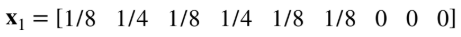
\includegraphics[width=0.8\linewidth]{images/bag_of_words.png}
\end{center}

\subsection{Images: Visual BoW}
Extract patches $\to$ cluster into $D$ visual words $\to$ count $\to$ normalize $\Rightarrow x_i\in\R^D$.

\subsection{Missing Data}
\kv{Drop}{loses info}\\
\kv{Global mean}{fast, ignores class}\\
\kv{Class-conditioned mean}{best}

\subsection{Noise / Binning}
Sort $\to$ bins $\to$ replace by bin mean/median.

\section{Imbalanced Data}
\begin{prop}[title=Sampling Methods]
\textbf{Oversampling:} + minority; naive duplication can overfit; SMOTE-like neighbors can add noise.\\
\textbf{Undersampling:} - majority; random removal may discard important samples; remove redundancy.
\end{prop}

\begin{thm}[title=Cost-sensitive Risk]
\[
R=\frac1N\sum_i\beta_i\ell(\hat y_i,y_i)
\]
Do not optimize \(\beta_i\): trivial 0-loss solutions.
\end{thm}

\section{Neural Networks}
\begin{center}
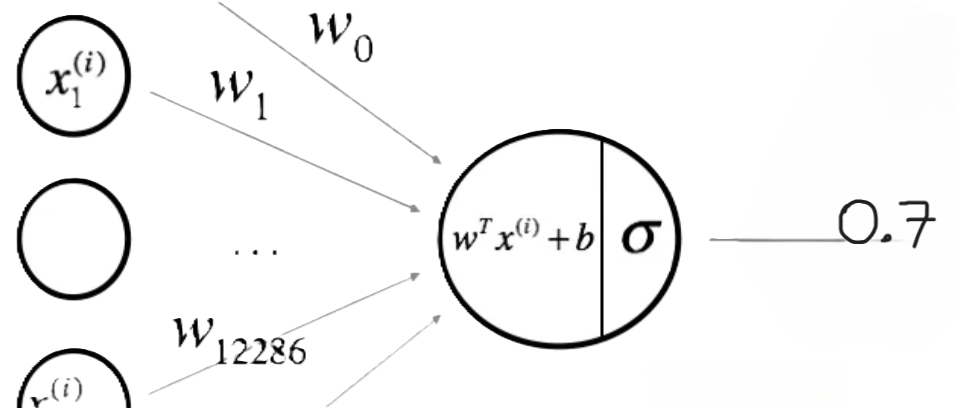
\includegraphics[width=0.9\linewidth]{images/mlp-zoom.png}
\end{center}

\begin{prop}[title=Backpropagation]
For neuron \(k\) in layer \(l\):
\[
a^{(k)}_{(l)}=\sum_jW^{(k,j)}_{(l)}z^{(j)}_{(l-1)},\quad
z^{(k)}_{(l)}=f(a^{(k)}_{(l)})
\]
\[
\delta^{(k)}_{(l)}=\frac{\partial\ell_i}{\partial a^{(k)}_{(l)}},\qquad
\frac{\partial\ell_i}{\partial W^{(k,j)}_{(l)}}=
\delta^{(k)}_{(l)}z^{(j)}_{(l-1)}
\]
\end{prop}

\begin{defn}[title=Mini-Batch SGD]
\[ W_k \leftarrow W_{k-1} - \eta\sum_{b=1}^{B}\nabla\ell_{(b,k)}(W_{k-1}) \]
$B$ = batch size. Full GD: $B=N$; SGD: $B=1$; mini-batch: $1<B<N$.
\end{defn}

\begin{prop}[title=SGD with Momentum]
\[
\nu\leftarrow\gamma\nu+\eta\nabla R(W),\qquad W\leftarrow W-\nu
\]
$\gamma>0$ adds inertia; accelerates if $\nabla$ is consistent.
\end{prop}

\begin{defn}[title=Neural Network Regularization]
\textbf{Dropout:} zero each neuron w.p.\ $p$ during train.\\
\textbf{Early stopping:} stop when val.\ loss starts rising.\\
\textbf{Weight decay:} $+\lambda\|W\|_F^2$ in loss (L2 for NNs).\\
\textbf{Data augmentation:} flip/crop/rotate.
\end{defn}

\section{Convolutional Neural Network (CNN)}

\begin{center}
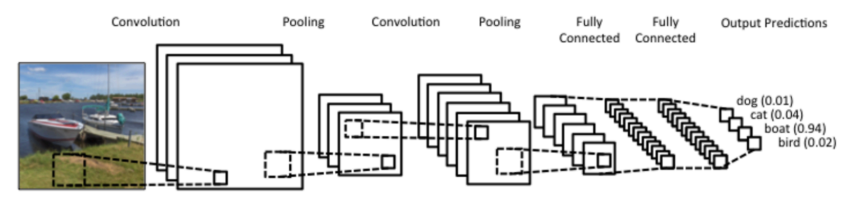
\includegraphics[width=\linewidth]{images/CNN_details.png}
\end{center}

\begin{defn}[title=Output Size \& Params]
Output size: \(\lfloor(W-F+2P)/S\rfloor+1\).\\
Same padding: \(P=(F-1)/2\).\\
Params: \((F^2C_{\mathrm{in}}+1)\times C_{\mathrm{out}}\) (far fewer than FC).
\end{defn}

\begin{prop}[title=Transposed Conv]
It upsamples: output size \((W{-}1)S+F\).
\end{prop}

\begin{warn}[title=CNN Tricks]
Convs: translation equivariance.\\
Pooling/stride: downsampling + robustness.
\end{warn}

\begin{center}
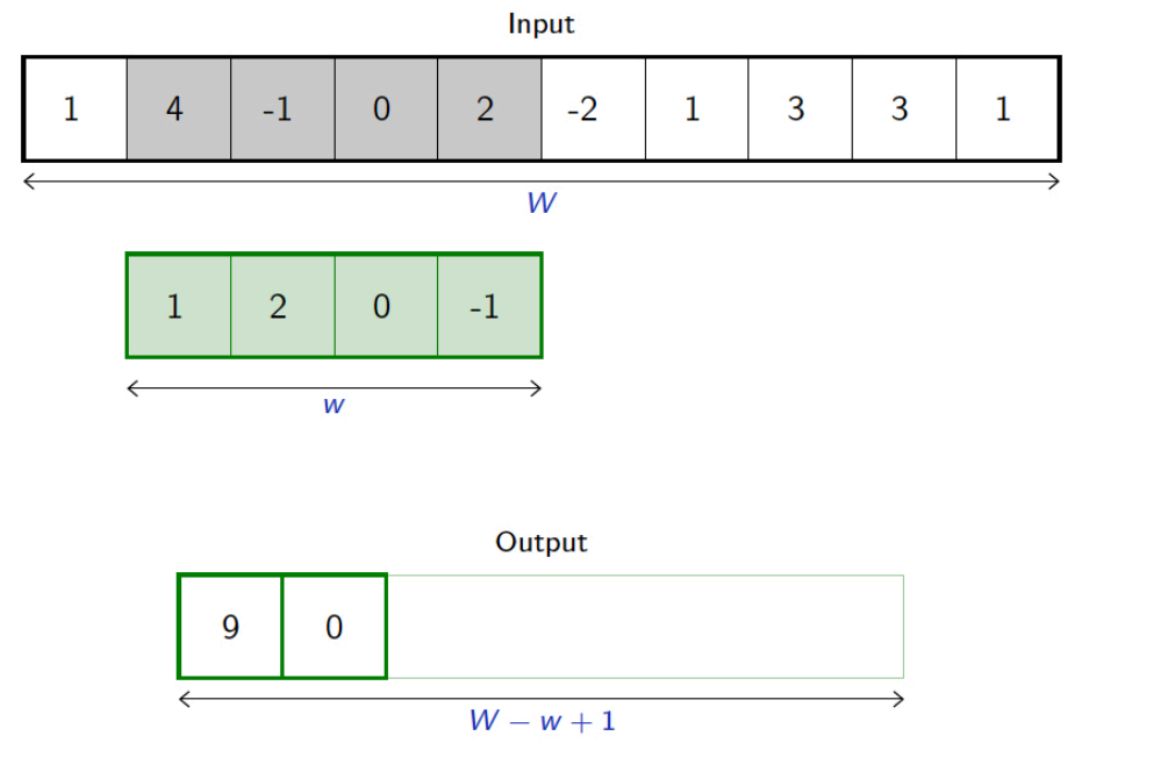
\includegraphics[width=0.7\linewidth]{images/conv.png}
\end{center}

\begin{center}
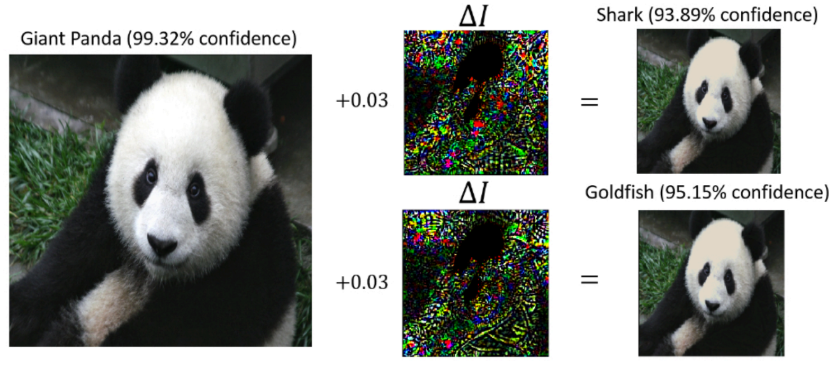
\includegraphics[width=0.9\linewidth]{images/panda.png}
\end{center}

\section{Dimensionality Reduction}
\textit{Limitation:} only captures linear structure.

\begin{prop}[title=PCA Projection]
\[
\bar x=\frac1N\sum_i x_i,\qquad
y_i=W^T(x_i-\bar x),\quad W^TW=I_d
\]
Covariance:
\[
C=\frac1N\sum_i(x_i-\bar x)(x_i-\bar x)^T
\]
1D objective:
\[
\max_{\|w\|=1}w^TCw\quad\Rightarrow\quad Cw=\lambda w
\]
\end{prop}

\begin{prop}[title=PCA Reconstruction]
\[
\hat x_i=\bar x+Wy_i=\bar x+WW^T(x_i-\bar x)
\]
PCA minimizes reconstruction error among linear orthogonal projections. (Uncorrelated = covariance matrix diagonal in the new space). Keep \(d\) such that:
\[
\sum_{j=1}^{d}\lambda_j\ge0.9\sum_{k=1}^{D}\lambda_k
\]
\end{prop}

\begin{warn}[title=Reduces cost and can regularize]
\textbf{Invariant under addition} ($x_i+c$): mean shifts by $c$, covariance unchanged $\Rightarrow$ same eigenvectors/values.\\
\textbf{Not invariant under scaling} ($Dx_i$): covariance changes $\Rightarrow$ eigenvectors change. Normalize first.
\end{warn}

\section{Kernel PCA + Autoencoders}
No reconstruction. \textit{When:} non-linear structure in data.

\begin{prop}[title=Kernel PCA]
\[
x_i\mapsto\phi(x_i),\qquad K_{ij}=k(x_i,x_j)
\]
Representer:
\[
w=\sum_{j=1}^{N}a_j\phi(x_j),\qquad Ka=\lambda Na
\]
Projection:
\[
y_i=\phi(x_i)^Tw=\sum_{j=1}^{N}a_jk(x_i,x_j)
\]
Kernel PCA maps high \(\to\) low, but unlike PCA it does not naturally provide low \(\to\) high reconstruction.
\end{prop}

Reconstruction possible. \textit{When:} non-linear structure; need encoder \& decoder; large data.

\begin{defn}[title=Autoencoder]
\textbf{Encoder:} input \(\to\) latent representation. \textbf{Decoder:} latent \(\to\) reconstruction. Train with:
\[
R=\frac1N\sum_i\|\hat x_i-x_i\|^2
\]
Non-convex; trained by SGD/backprop. Decoder gives low/latent \(\to\) output mapping, so latent vectors can generate samples.
\end{defn}

\begin{prop}[title=Variants]
\textbf{Deep AE:} stacked layers \(z^{(j)}=f^{(j)}(W_{(j)}^Tz^{(j-1)})\).\\
\textbf{Denoising AE:} corrupt input, reconstruct clean input; learns robust representation.
\end{prop}

\begin{center}
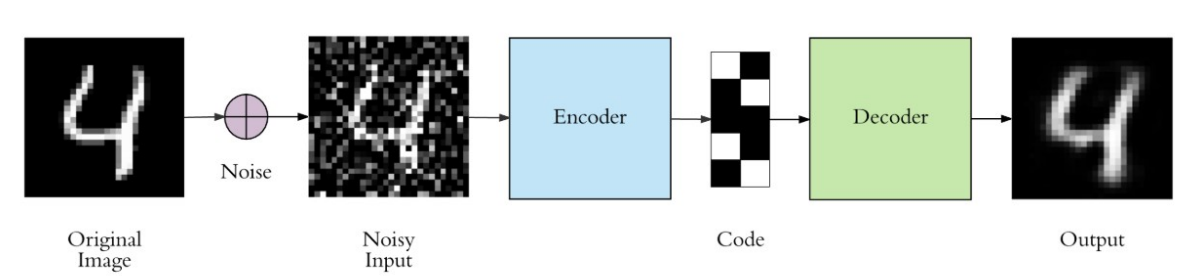
\includegraphics[width=\linewidth]{images/denoising_autoencoder.png}
\end{center}

\iffalse
\section{LDA + Clustering}
\begin{prop}[title=Fisher LDA]
Supervised dimensionality reduction using class labels. Want low within-class variance and high between-class separation.
\[
S_W=\sum_{c=1}^{C}\sum_{i\in c}(x_i-\mu_c)(x_i-\mu_c)^T
\]
\[
S_B=\sum_{c=1}^{C}N_c(\mu_c-\bar x)(\mu_c-\bar x)^T
\]
\[
J(w)=\frac{w^TS_Bw}{w^TS_Ww},\qquad
S_Bw=\lambda S_Ww
\]
Take eigenvectors with largest eigenvalues. At most \(C-1\) useful dimensions because \(\mathrm{rank}(S_B)\le C-1\).
\end{prop}

\begin{defn}[title=PCA vs LDA]
PCA/eigenfaces minimize reconstruction error and may keep nuisance variation (e.g. illumination). LDA/fisherfaces keep discriminative directions for labels/classes.
\end{defn}
\fi

\section{K-means}
\textit{Complexity:} $O(NKD)$ per iteration.

\begin{prop}[title=Problem + Algorithm]
Unsupervised clustering into \(K\) groups with compact clusters.
\begin{enumerate}
\item Initialize centers \(\mu_1,\ldots,\mu_K\).
\item Assign each \(x_i\) to nearest \(\mu_k\).
\item Update each \(\mu_k\) as mean of assigned points.
\item Repeat until assignments/centers stop changing.
\end{enumerate}
\end{prop}

\begin{warn}[title=K-means Tricks]
Initialization matters; run multiple initializations. Euclidean distance makes feature scaling crucial. Elbow method helps choose \(K\).\\
K-means exploits compactness; fails on non-compact clusters such as concentric circles.
\end{warn}

\section{NLP, RNNs, Attention}
\begin{defn}[title=Word Representations]
\textbf{Word2Vec}: dense \(\R^d\) embeddings trained self-supervised from context; similar words \(\approx\) nearby vectors (king\(-\)man\(+\)woman\(\approx\)queen).
\end{defn}

\begin{center}
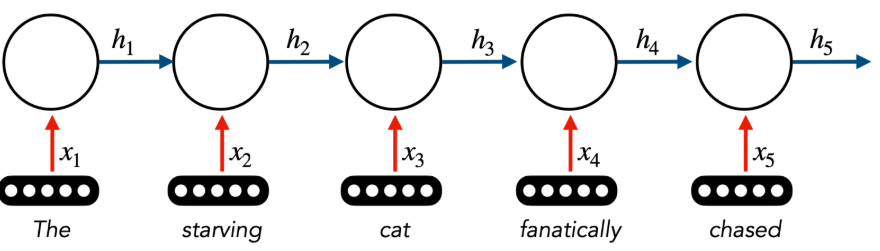
\includegraphics[width=0.95\linewidth]{images/rnn.png}
\end{center}

\begin{center}
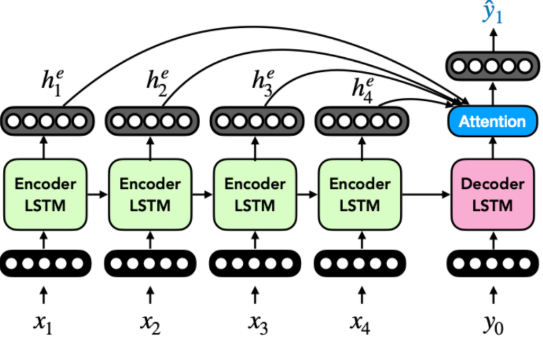
\includegraphics[width=0.7\linewidth]{images/attention.png}
\end{center}

\section{Transformers}
\begin{center}
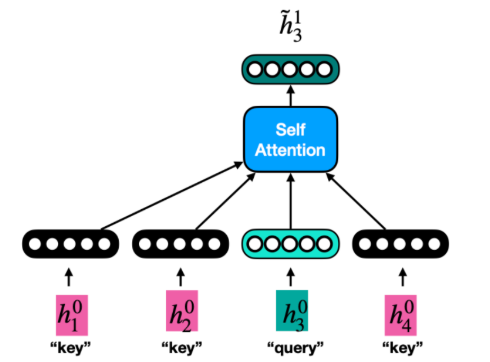
\includegraphics[width=0.8\linewidth]{images/self_attention.png}
\end{center}

\begin{prop}[title=Transformer Blocks]
Transformer encoder/decoder are stacks of blocks with multi-head attention, feed-forward layers, and Add \& Norm. Main advantage over RNNs: self-attention can process inputs in parallel instead of sequentially.
\end{prop}

\begin{defn}[title=Decoder Details]
Masked self-attention prevents attending to future tokens. Cross-attention in the decoder attends over encoder outputs. GPT is a decoder transformer using masked multi-head self-attention and no cross-attention.
\end{defn}

\begin{warn}[title=Common Checks]
RBF kernel has an infinite-dimensional feature view.\\
kNN works for regression and classification; \(k\) is not learned by GD.\\
K-means converges, but not always to the desired/global solution.\\
PCA components are ordered by eigenvalues; labels do not change PCA.
\end{warn}

\begin{defn}[title=Parameter Counting]
Fully connected layer \(n_{\mathrm{in}}\to n_{\mathrm{out}}\):
\[
\#\mathrm{params}=(n_{\mathrm{in}}+1)n_{\mathrm{out}}
\]
Convolution layer with kernel \(H_K\times W_K\), \(C_{\mathrm{in}}\) input channels, \(C_{\mathrm{out}}\) filters:
\[
\#\mathrm{params}=(H_KW_KC_{\mathrm{in}}+1)C_{\mathrm{out}}
\]
\end{defn}

\vfill
\begin{center}
\textit{Bon courage.}
\end{center}

\end{multicols*}
\end{document}
